\documentclass[12pt]{article}
\usepackage[utf8]{inputenc}
\usepackage[letterpaper, margin=1in]{geometry}
\usepackage{graphicx}
\usepackage{mathptmx}
\usepackage{float}
\usepackage[cmex10]{amsmath}
\usepackage{amsthm,amssymb}
\usepackage{url}
\urlstyle{same} 
\def\UrlBreaks{\do\/\do-}
\usepackage{breakurl}
\usepackage{fancybox}
\usepackage{breqn}
\usepackage{array}
\usepackage{caption}
\usepackage{subcaption}
\usepackage{comment}
\usepackage[english]{babel}
\usepackage[acronym,nomain]{glossaries} % list of acronyms
\usepackage{xurl}
\usepackage{multicol}
\usepackage{multirow}
\usepackage{mathptmx}
\usepackage{float}
\usepackage{lipsum}
\usepackage{framed}
\usepackage[T1]{fontenc}
\usepackage[pdfpagelabels,pdfusetitle,colorlinks=false,pdfborder={0 0 0}]{hyperref}
\usepackage{algorithm}
\usepackage{algpseudocode}
\usepackage{tabularx}
\usepackage{wrapfig}

% draw a frame around given text
\newcommand{\framedtext}[1]{%
	\par%
	\noindent\fbox{%
		\parbox{\dimexpr\linewidth-2\fboxsep-2\fboxrule}{#1}%
	}%
}

\renewcommand{\arraystretch}{1.2}

\sloppy

\newcolumntype{C}[1]{>{\centering\let\newline\\\arraybackslash\hspace{0pt}}m{#1-2\tabcolsep}}

\usepackage[%
backend=bibtex,     % biber or bibtex
%style=authoryear,    % Alphabeticalsch
style=numeric-comp,  % numerical-compressed
sorting=none,        % no sorting
sortcites=true,      % some other example options ...
block=none,
indexing=false,
citereset=none,
isbn=true,
url=true,
doi=true,           % prints doi
natbib=true,         % if you need natbib functions
]{biblatex}
\addbibresource{./sources/sources.bib,}  % better than \bibliography

\title{Increasing \gls{bev} Access in California via Capability and Risk Sensitive \gls{evse} Targeted Deployment}
\author{Aaron I. Rabinowitz, Vaishnavi Karanam, Gil Tal?, Alan Jenn?}
\date{}

\newacronym{ghg}{GHG}{Green-House Gas}
\newacronym{fe}{FE}{Fuel Economy}
\newacronym{ee}{EE}{Energy Economy}
\newacronym{epa}{EPA}{Environmental Protection Agency}
\newacronym{oem}{OEM}{Original Equipment Manufacturer}
\newacronym{ice}{ICE}{Internal Combustion Engine}
\newacronym{icv}{ICV}{Internal Combustion Vehicle}
\newacronym{icev}{ICEV}{Internal Combustion Engine Vehicle}
\newacronym{em}{EM}{Electric Motor}
\newacronym{hev}{HEV}{Hybrid Electric Vehicle}
\newacronym{ev}{EV}{Electric Vehicle}
\newacronym{phev}{PHEV}{Plug-in Hybrid Electric Vehicle}
\newacronym{lrphev}{LR-PHEV}{Long Range PHEV}
\newacronym{srphev}{SR-PHEV}{Short Range PHEV}
\newacronym{mhev}{MHEV}{Mild Hybrid Electric Vehicle}
\newacronym{pev}{PEV}{Plug-in Electric Vehicle}
\newacronym{bev}{BEV}{Battery Electric Vehicle}
\newacronym{cbev}{CBEV}{City BEV}
\newacronym{afv}{AFV}{Alternative Fuel Vehicle}
\newacronym{fcev}{FCEV}{Fuel Cell Electric Vehicle}
\newacronym{cav}{CAV}{Connected Autonomous Vehicle}
\newacronym{fc}{FC}{Fuel Consumption}
\newacronym{ec}{EC}{Energy Consumption}
\newacronym{dtto}{DTTO}{Discrete Time Trajectory Optimization}
\newacronym{udto}{UDTO}{Uniformly Discretized Trajectory Optimization}
\newacronym{sto}{STO}{Spline Trajectory Optimization}
\newacronym{rbed}{RBED}{Rules-Based Eco-Driving}
\newacronym{cidm}{CIDM}{Cooperative Intelligent Driver Model}
\newacronym{idm}{IDM}{Intelligent Driver Model}
\newacronym{soc}{SOC}{State of Charge}
\newacronym{ocp}{OCP}{Optimal Control Problem}
\newacronym{ttc}{TTC}{Time-To-Collision}
\newacronym{dp}{DP}{Dynamic Programming}
\newacronym{ga}{GA}{Genetic Algorithm}
\newacronym{sdm}{SDM}{Smart Driver Model}
\newacronym{v2i}{V2I}{Vehicle to Infrastructure}
\newacronym{v2v}{V2V}{Vehicle to Vehicle}
\newacronym{v2x}{V2X}{Vehicle to Everything}
\newacronym{hil}{HIL}{Hardware In Loop}
\newacronym{pso}{PSO}{Particle Swarm Optimization}
\newacronym{dt}{DT}{Direct Transcription}
\newacronym{oedt}{OEDT}{Optimal Eco-Driving Trace}
\newacronym{fods}{FODS}{Forward Object Detection System}
\newacronym{cas}{CAS}{Collision Aviodance System}
\newacronym{acc}{ACC}{Adaptive Cruise Control}
\newacronym{obu}{OBU}{On-Board Unit}
\newacronym{rsu}{RSU}{Road-Side Unit}
\newacronym{sae}{SAE}{Society of Automotive Engineers}
\newacronym{adas}{ADAS}{Advanced Driver Assistance System}
\newacronym{edc}{EDC}{Eco-Driving Control}
\newacronym{lv}{LV}{Lead Vehicle}
\newacronym{ss}{SS}{Segment Speeds}
\newacronym{hs}{HS}{Historical Speeds}
\newacronym{spat}{SPAT}{Signal Phase and Timing}
\newacronym{map}{MAP}{Positions of Subsequent Traffic Lights}
\newacronym{al2n}{AL2N}{Acceleration L\textsuperscript{2} Norm}
\newacronym{rpc}{RPC}{Road Power Cost}
\newacronym{bpc}{BPC}{Battery Power Cost}
\newacronym{fecc}{FECC}{Fitted Equivalent Consumption Cost}
\newacronym{ipopt}{IPOPT}{Interior-Point Optimization}
\newacronym{dtnlp}{DTNLP}{Discreet-Time Non-Linear Programming}
\newacronym{snlp}{SNLP}{Spline Non-Linear Programming}
\newacronym{sga}{SGA}{Spline Genetic Algorithm}
\newacronym{spso}{SPSO}{Spline Particle Swarm Optimization}
\newacronym{2sdp}{2SDP}{2 State Dynamic Programming}
\newacronym{aos}{AOS}{Approximate Optimal Spline}
\newacronym{pchip}{PCHIP}{Piecewise Cubic Hermitic Interpolation Polynomial}
\newacronym{nrel}{NREL}{National Renewable Energy Laboratory}
\newacronym{fastsim}{FASTSim}{Future Automotive Systems Technology Simulator}
\newacronym{mfei}{MFEI}{Mean Fuel Economy Improvement}
\newacronym{pas}{PAS}{Percent Acceptable Solutions}
\newacronym{mrt}{MRT}{Mean Run-Time}
\newacronym{mpc}{MPC}{Model Predictive Control}
\newacronym{adp}{ADP}{Approximate Dynamic Programming}
\newacronym{rl}{RL}{Reinforcement Learning}
\newacronym{mbrl}{MBRL}{Model Based Reinforcement Learning}
\newacronym{nlp}{NLP}{Non-Linear Programming}
\newacronym{nhtsa}{NHTSA}{National Highway Traffic Safety Administration}
\newacronym{aeb}{AEB}{Automatic Emergency Braking}
\newacronym{tsdc}{TSDC}{Transportation Secure Data Center}
\newacronym{anl}{ANL}{Argonne National Lab}
\newacronym{d3}{D\textsuperscript{3}}{Downloadable Dynamometer Database}
\newacronym{cd}{C\textsubscript{D}}{Coefficient of Drag}
\newacronym{crr}{C\textsubscript{RR}}{Coefficient of Rolling Resistance}
\newacronym{mape}{MAPE}{Mean Absolute Percentage Error}
\newacronym{evse}{EVSE}{Electric Vehicle Supply Equipment}
\newacronym{ld}{LD}{Light Duty}
\newacronym{md}{MD}{Medium Duty}
\newacronym{hd}{HD}{Heavy Duty}
\newacronym{mdhd}{MD/HD}{Medium Duty / Heavy Duty}
\newacronym{inrix}{INRIX}{}
\newacronym{epri}{EPRI}{Electric Power Research Institute}
\newacronym{nhts}{NHTS}{National Highway Transportation Survey}
\newacronym{usa}{USA}{United States of America}
\newacronym{sof}{SOF}{State of Fuel}
\newacronym{hc}{HC}{Home Charging}
\newacronym{bc}{BC}{Battery Capacity}
\newacronym{dcl}{DCL}{Destination Charger Likelihood}
\newacronym{ercr}{ERCR}{En-Route Charging Rate}
\newacronym{ercp}{ERCP}{En-Route Charging Penalty}
\newacronym{ftc}{FTC}{Fuel Tank Capacity}
\newacronym{ftp}{FTP}{Fuling Time Penalty}
\newacronym{psrc}{PSRC}{Puget Sound Regional Council}
\newacronym{bts}{BTS}{Bureau of Transportation Statistics}
\newacronym{happ}{HAPP}{Household Activity Pattern Problem}
\newacronym{chts}{CHTS}{California Houslehold Travel Survey}
\newacronym{dcfc}{DCFC}{DC Fast Charging}
\newacronym{liion}{Li-Ion}{Lithium-Ion}
\newacronym{lvl2}{LVL 2}{DC Level 2}
\newacronym{oems}{OEMS}{Optimal Energy Management Strategies}
\newacronym{poems}{POEMS}{Predictive Optimal Energy Management Strategies}
\newacronym{vpoems}{VP-OEMS}{Velocity Prediction enabled Optimal Energy Management Strategies}
\newacronym{gnss}{GNSS}{Global Navigational Satellite System}
\newacronym{obd2}{OBD-II}{On-Board Diagnostics II}
\newacronym{csu}{CSU}{Colorado State University}
\newacronym{wes}{WES}{Weight Efficiency Score}
\newacronym{gvwr}{GVWR}{Gross Vehicle Weight Rating}
\newacronym{fha}{FHA}{Federal Highway Administration}
\newacronym{vius}{VIUS}{Vehicle Inventory and Use Survey}
\newacronym{eod}{EOD}{End of Day}
\newacronym{osrm}{OSRM}{Open-Source Routing Machine}
\newacronym{vrp}{VRP}{Vehicle Routing Problem}
\newacronym{evrp}{EVRP}{Electric Vehicle Routing Problem}
\newacronym{tsp}{TSP}{Traveling Salesman Problem}
\newacronym{can}{CAN}{Controller Area Network}
\newacronym{lstm}{LSTM}{Long Short-Term Memory}
\newacronym{ann}{ANN}{Artificial Neural Network}
\newacronym{ml}{ML}{Machine Learning}
\newacronym{fcdp}{FC-DP}{Full Cycle Dynamic Programming}
\newacronym{ppmpc}{PP-MPC}{Perfect Prediction Model Predictive Control}
\newacronym{rpmpc}{RP-MPC}{Real Prediction Model Predictive Control}
\newacronym{cvmpc}{CV-MPC}{Constant Velocity Model Predictive Control}
\newacronym{mae}{MAE}{Mean Absolute Error}
\newacronym{fsmvrp}{FSMVRP}{Fleet Size and Mix Vehicle Routing Problem}
\newacronym{mcvrp}{MCVRP}{Monte-Carlo Vehicle Routing Problem}
\newacronym{ppf}{PPF}{Percent Point Function}
\newacronym{ccdng}{CCDNG}{Completely Connected Directional Network Graph}
\newacronym{sho}{SHO}{Spline Heuristic-Optimal}
\newacronym{npv}{NPV}{Net Present Value}
\newacronym{tco}{TCO}{Total Cost of Ownership}
\newacronym{mtk}{MTK}{Metric-Ton-Kilometer}
\newacronym{lco}{LCO}{Levelized Cost of Ownership}
\newacronym{lcod}{LCOD}{Levelized Cost of Driving}
\newacronym{sme}{SME}{Subject Matter Expert}
\newacronym{doe}{DOE}{Deparment of Energy}
\newacronym{vmt}{VMT}{Vehicle Miles Traveled}
\newacronym{dot}{DOT}{Department of Transportation}
\newacronym{ltl}{LTL}{Less Than Truckload}
\newacronym{lpcp}{LPCP}{Lost Payload Capacity Portion}
\newacronym{chaas}{ChaaS}{Charging as a Service}
\newacronym{tou}{TOU}{Time of Use}
\newacronym{ocs}{OCS}{Optimal Charging Strategy}
\newacronym{soe}{SOE}{State of Energy}
\newacronym{ltp}{LTP}{Lost Time Portion}
\newacronym{yd}{YD}{Yearly Distance}
\newacronym{dd}{DD}{Daily Distance}
\newacronym{vnr}{VNR}{Vehicle Nominal Range}
\newacronym{nyo}{NYO}{Number of Years of Ownership}
\newacronym{ap}{AP}{Age at Purchase}
\newacronym{dpm}{DPM}{Diesel Price Multiplier}
\newacronym{epm}{EPM}{Electricity Price Multiplier}
\newacronym{evsep}{EVSEP}{EVSE Premium}
\newacronym{pe}{PE}{Payload Exemption}
\newacronym{bpp}{BPP}{Battery Pack Pricing}
\newacronym{my}{MY}{Model Year}
\newacronym{ipfn}{IPFN}{Iterative Proportional Fitting with N dimensions}
\newacronym{dco}{DCO}{Discretized Control Optimization}
\newacronym{pto}{PTO}{Polynomial Trajectory Optimization}
\newacronym{slsqp}{SLSQP}{Sequential Least Squares Programming}
\newacronym{aer}{AER}{All Electric Range}
\newacronym{msrp}{MSRP}{Manufacturer Recommended Sales Price}
\newacronym{afdc}{AFDC}{Alternative Fuels Data Center}
\newacronym{uf}{UF}{Utility Factor}
\newacronym{hov}{HOV}{Hich Occupancy Vehicle}
\newacronym{lp}{LP}{Linear Problem}
\newacronym{qp}{QP}{Quadratic Problem}
\newacronym{sp}{SP}{Stochastic Problem}
\newacronym{slp}{S-LP}{Stochastic Linear Problem}
\newacronym{milp}{MILP}{Mixed Integer Linear Problem}
\newacronym{smilp}{S-MILP}{Stochastic Mixed Integer Linear Problem}
\newacronym{los}{LOS}{Level of Service}
\newacronym{v2s}{V2S}{Vehicle-to-Structure}
\newacronym{v2g}{V2G}{Vehicle-to-Grid}
\newacronym{gacm}{GACM}{Grid-Aware Charge Management}
\newacronym{iso}{ISO}{Independent System Operator}
\newacronym{dcopf}{DC-OPF}{DC Optimal Power Flow}
\newacronym{lmp}{LMP}{Location Marginal Price}
\newacronym{gcc}{GCC}{Giant Connected Component}
\newacronym{hjb}{HJB}{Hamilton-Jacobi-Bellman}
\newacronym{pdf}{PDF}{Probability Distribution Function}
\newacronym{scram}{SCRAM}{Stochastic Cost with Risk Allowance Minimization}
\newacronym{scramd}{SCRAM-D}{SCRAM-Dijkstra}
\newacronym{scramb}{SCRAM-B}{SCRAM-Bellman}
\newacronym{rsic}{RSIC}{Range-Sensitive Information Centrality}
\newacronym{rsbc}{RSBC}{Range-Sensitive Betweenness Centrality}
\newacronym{ras}{RAS}{Range Addition Station}

\makeglossaries

\begin{document}

\maketitle

\section*{Abstract}

A well designed transportation system is one which provides sufficient access from residences to opportunities and from production sited to warehousing sites and demand sites. Increasingly, climate action goals require that more transportation load be shifted to less \gls{ghg} intensive modes among which are \glspl{bev}. While \glspl{bev} use the same roads as \glspl{icev} they draw energy from a separate network of stations which neither as robust as nor coincident to the \gls{icev} fueling network, a consequence of the different current and historical economics of both. Insufficiency and unreliability of public DC \gls{evse} which is primarily used for charging on long itineraries mean that \gls{bev} drivers, depending on vehicle range and risk attitude, may opt for less direct paths with lower charging risk, opt for a more \gls{ghg} intensive mode, or abandon an itinerary. Holistically, the transportation system provides less access to \glspl{bev} for distant pairs. This project develops methods and tools to optimize deployment of future \gls{evse} to mitigate the issue. Methods herein are based on range and charging risk sensitive optimal routing between O/D pairs subject to the locations and usability rates of \gls{evse}. These methods and tools may be used by policy makers to directly evaluate the impact of proposed stations on \gls{bev} transportation access.

\section*{Description of Proposed Research}

\subsection*{Project Purpose}

This project seeks to support CalTrans's goals of creating a quantitative framework of assessment for access benefits provided by \gls{ev} support projects in general and to propose guidelines for future development.

The access provided by the California road transportation system for \glspl{bev} is different than that for \glspl{icev} due to vehicular and support station network characteristics. Access is worse for \glspl{bev} due to a lower density of support stations, lower station usability rates, and the expected time required to charge. The disparity of access is different for each vehicle based on its range and charging characteristics as well as for each driver based on risk attitude. Insufficient access will motivate trip cancelations or mode switches, most often to \gls{icev} or air travel. This situation may be mitigated but not resolved or reversed through the careful allocation of \gls{evse} deployment incentives. Evaluation methods for potential charging stations should consider their access impact network-wide in a manner which accounts for distributions of vehicle type, charge event outcomes, and driver risk attitude. The proposed method accomplishes these goals by computing most-likely (optimal) all-pairs routes between Places (Census Bureau definition) within California or some subset subject to risk attitude. Access is expected to be uneven across the state and proportional to wealth.

Specific negative outcomes which may motivate drivers are out-of-range events wherein the driver must be towed to a charger and long delays due to queuing. The probabilities of both outcomes are a function of the usability rates of chargers along a driver's route where a usable charger is one which is functional, accessible, and available. More common and more reliable chargers will result in higher usability rates at first but may become less usable due to induced demand. Drivers may elect for less direct routes with higher expected charger usability rates in order to avoid negative outcomes. Drivers may decide to not attempt trips where no route which meets maximum cost and minimum reliability requirements exists. Thus access failures may be partial (trip is more costly) or complete (trip is infeasible). Partial and complete access failures are both undesirable but partial failures are preferable and there may be substantial variations in severity among partial failures.

Although, ultimately the state of infrastructure drives experience, individual perceptions will differ. Drivers will each have different risk attitudes. Risk attitude is the weighting of outcomes as a function of severity. Risk-averse drivers will over-value low-probability high-severity outcomes. Risk-neutral drivers will evenly value all outcomes. Risk-accepting drivers will over-value low-probability low-severity outcomes. The risk attitude of a driver can be modeled, for a large sample of outcomes, using the superquantile function of the empirical distribution of outcomes. Thus optimal routes can be computed for a given driver/car subject to risk attitude using a Monte-Carlo Dijkstra routing algorithm wherein precedence is determined by comparing superquantile values. The result will be optimal-feasible routes for all pairs of selected Places where possible given charger locations and usability rates. The exact same method can be used to compute optimal-feasible routes for all pairs for \glspl{icev} using different data. Comparison between the optimal-feasible routes will reveal the access disparity. Products of this project will include reports, research papers, outreach material, webinar(s), and open-source tools.

\subsection*{Relevance to NCST Theme(s)}

This project is relevant to the NCST themes of infrastructure provision and vehicle electrification. Reducing the access gap between \glspl{bev} and \glspl{icev} will both increase \gls{bev} mode share and improve \gls{bev} adoption. Replacing \gls{icev} miles with less \gls{ghg} intensive \gls{ev} miles will reduce overall system \gls{ghg} intensity for equivalent travel demand.

\subsection*{Relevance to Caltrans Priorities}

This project directly addresses Caltrans's research area "Accessibility Changes as a Result of Projects that Support Electric Vehicles" as defined in Appendix B - Caltrans Research Needs for FY 2024-2025.

\subsection*{Equity Considerations of the Proposed Research}

The analysis framework and tool proposed is inherently geo-spatial and serves to quantify access for geographically defined communities. The impacts of every charger installed in the state can be assessed for every community in the state. The impacts of charger deployment can be, thus, accurately, computed for DACs as defined by Cal Enviro Screen or other geo-spatial tools.

\subsection*{Methodology / Scope of Work}

The proposed project will consist of three phases: data collection, tool development, and publication/reporting. The data collection phase will be minimal and will not require the acquisition of any new dataset. All data used will be publicly available such that the analysis tool can be used by any interested party in any region. The bulk of the effort will be devoted to tool development which will entail method refinement and the distribution of open-source applications. The final phase will involve generation and publication of results which will be both methodology and impact focused.

\subsubsection*{Data}

The proposed analysis framework is inherently geo-spatial and relies on sizes and locations of populations, travel between said locations, locations of public \gls{evse}, \gls{ev} ownership rates for locations, and a map of the road network which connects the mentioned entities. All of this data can be derived from publicly available sources. The locations of California's cities and towns (places) can be pulled from the US Census Bureau's \gls{gis} data server \cite{uscb_2023_doc, uscb_2023_files}. Locations and plug numbers for public \gls{evse} stations in North America can be pulled from \gls{afdc}'s data server \cite{afdc_2023}. Detailed regional road maps can be pulled from a variety of locations including the US Census Bureau \gls{gis} data server, ArcGIS Hub \cite{fhwa_2023}, and various maps APIs such as Google Maps, Bing Maps, and OpenStreetMap. Live and historical traffic conditions at points on the road map can be pulled from CalTrans's PeMS \cite{caltrans_2023} or the previously mentioned APIs. O/D pair travel volume information by mode can be pulled from \gls{fhwa}'s NextGen OD data server \cite{fhwa_2022}. All of the mentioned data sources are public and either entirely free or have a free tier. California's places, road map, and \gls{evse} stations are shown in Figure \ref{fig:atlas}.

\begin{figure}[H]
	\centering
	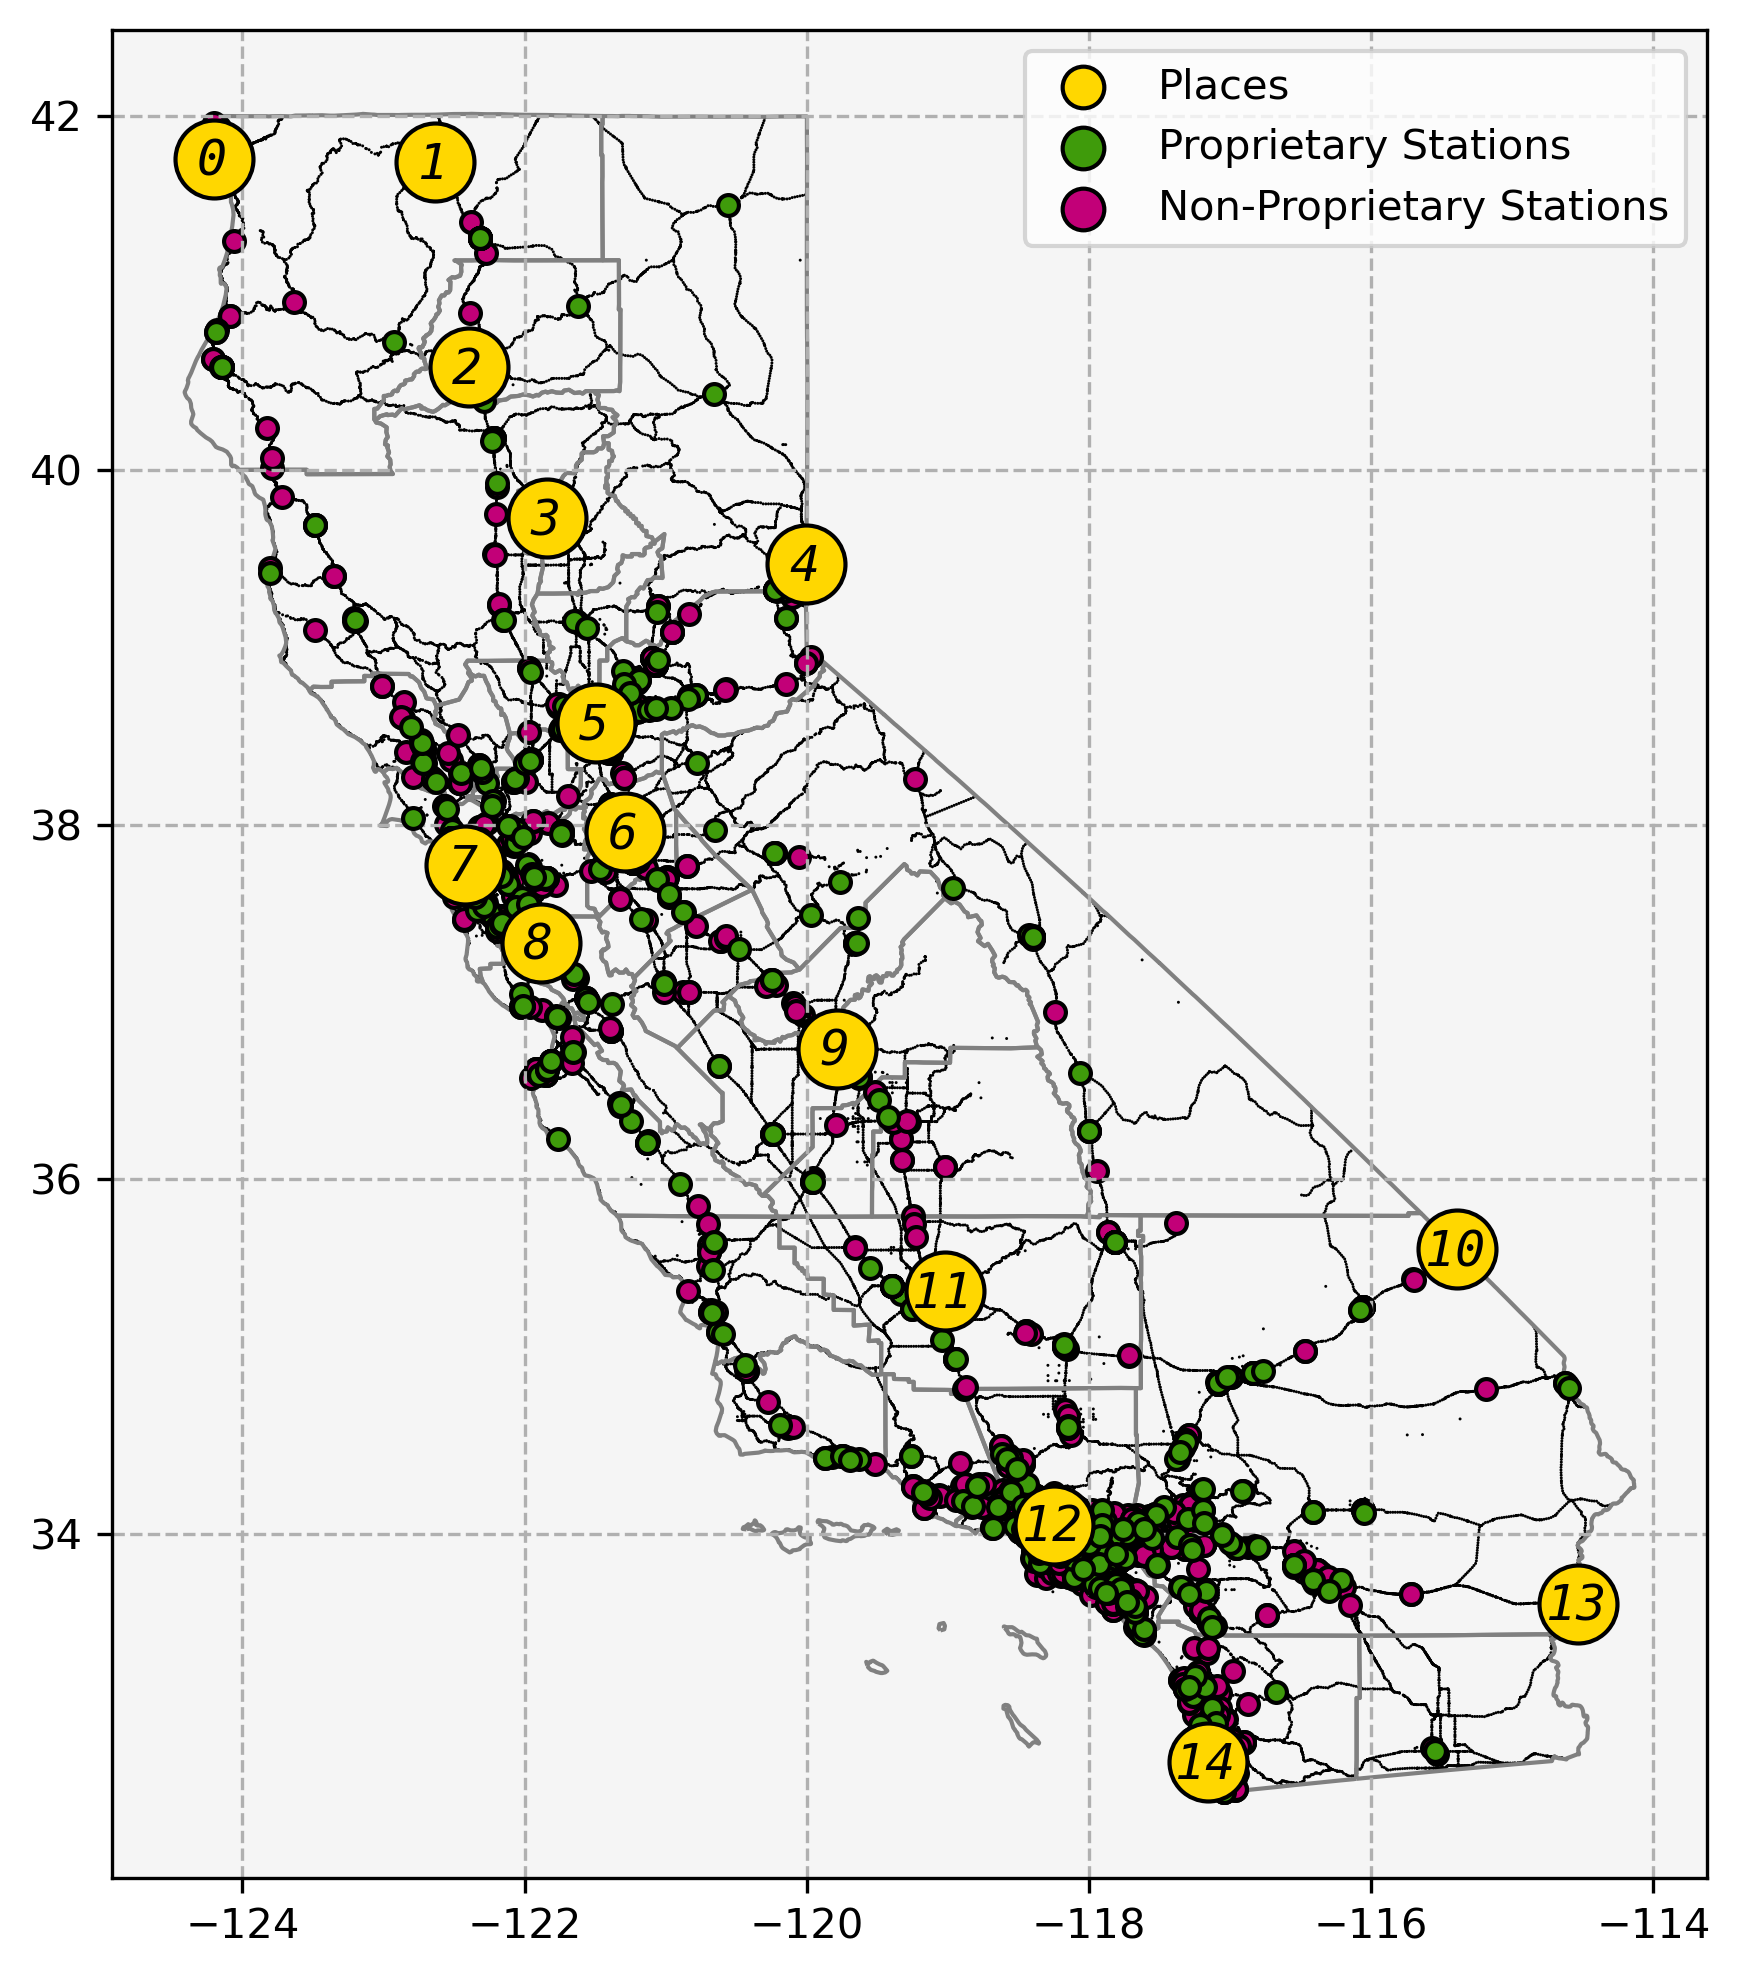
\includegraphics[width = \linewidth]{figs/California_Places_Chargers.png}
	\caption{Places, road map, and \gls{evse} stations in California}
	\label{fig:atlas}
\end{figure}

\subsubsection*{Tool Methodology}

The framework for transportation access herein considers the usability of the road transportation system for \gls{bev} users based on behavioral, infrastructural, and vehicular characteristics. Every person in a given region makes use of the same public \gls{evse} network which may be supplemented with several private chargers at home and work. Thus, for sufficiently long itineraries all drivers will be accommodated by the same infrastructure. However, as vehicles have differing ranges and drivers have different risk attitudes and locations of origin, the actual and perceived utility of the network will vary. The utility of the network, as experienced by identical cars and drivers and for every O/D pair, will be unequally effected by every single station addition and deletion as well as changes to reliability at existing stations.

The core method proposed is based on optimal routing for O/D pairs on a graph with stochastic node and edge costs. Routes are computed using a Monte-Carlo-Dijkstra method invented by the author. Path costs are a weighted sum of time, energy price, and complexity. Weights are tuned parameters and may vary by driver. As a consequence, the cost of a given route will be empirically distributed. For the purposes of comparison , a cost expectation is computed using a superquantile $p$ of the empirical distribution. Higher values of $p$ emphasize the most negative outcomes and, thus, represent conservative risk-attitude.

The method involves two steps. The first step of the method is to compute stochastic optimal paths for all pairs of entities (places and \gls{evse} stations) using the road map. The result is a directed multigraph where, due to the stochastic nature of the routing, all paths for a given pair whose cost is within the range of statistical insignificance from the lowest-cost-path are kept as options. The resulting multigraph is referred to as the atlas. In the second stage, optimal routes are computed for all place O/D pairs using the atlas subject to vehicle range limitations and stochasticity in charger usability at the \gls{evse} station nodes. Charger usability is based on assumed functionality rates availability at stations is based on expected queuing durations. Queuing duration estimation is an iterative process wherein time-varying charge event volumes at stations in iteration $n$ are computed from optimal routes from iteration $n-1$ until convergence. All routing is conducted sensitive to risk-attitude. The end result of the method is a tree of costs (time, distance, price, complexity) to all destinations from each origin for a given car and driver. The effects of station functionality rates and driver risk tolerance on network access are shown for a randomly generated atlas of 100 entities and 15 chargers in Figure \ref{fig:routing}.

\begin{figure}[H]
	\centering
	\begin{subfigure}{.5\linewidth}
		\centering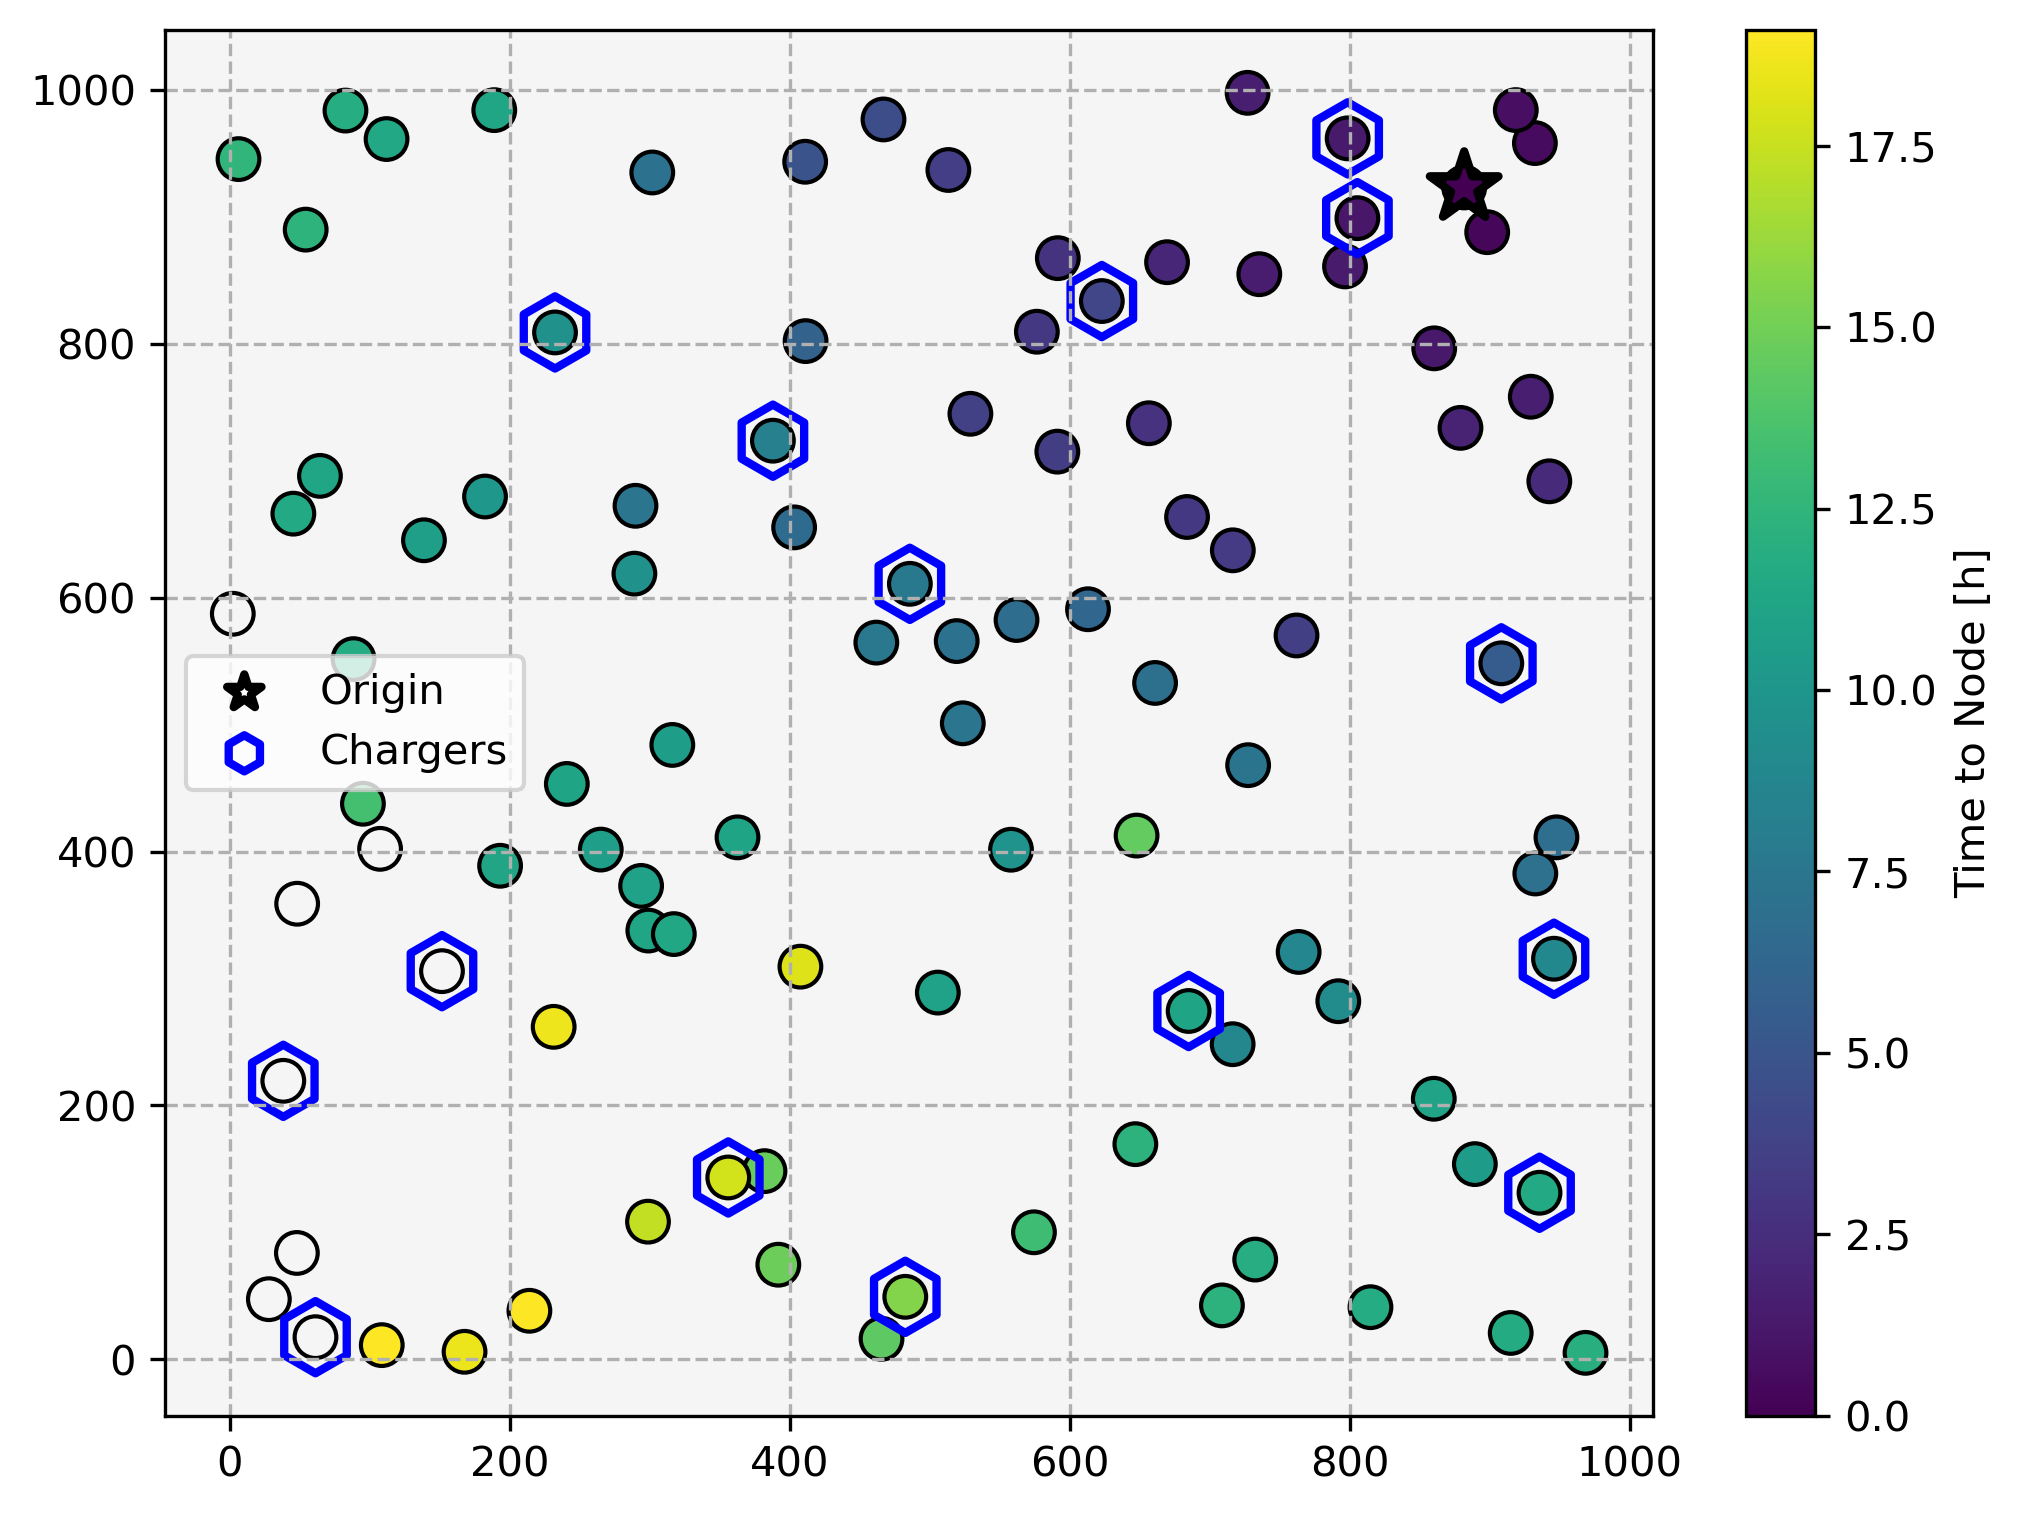
\includegraphics[width = \linewidth]{figs/parameter_factorial_00.png}
		\captionsetup{width=.8\linewidth}
		\caption{High risk tolerance and high charger usability}
	\end{subfigure}%
	\begin{subfigure}{.5\linewidth}
		\centering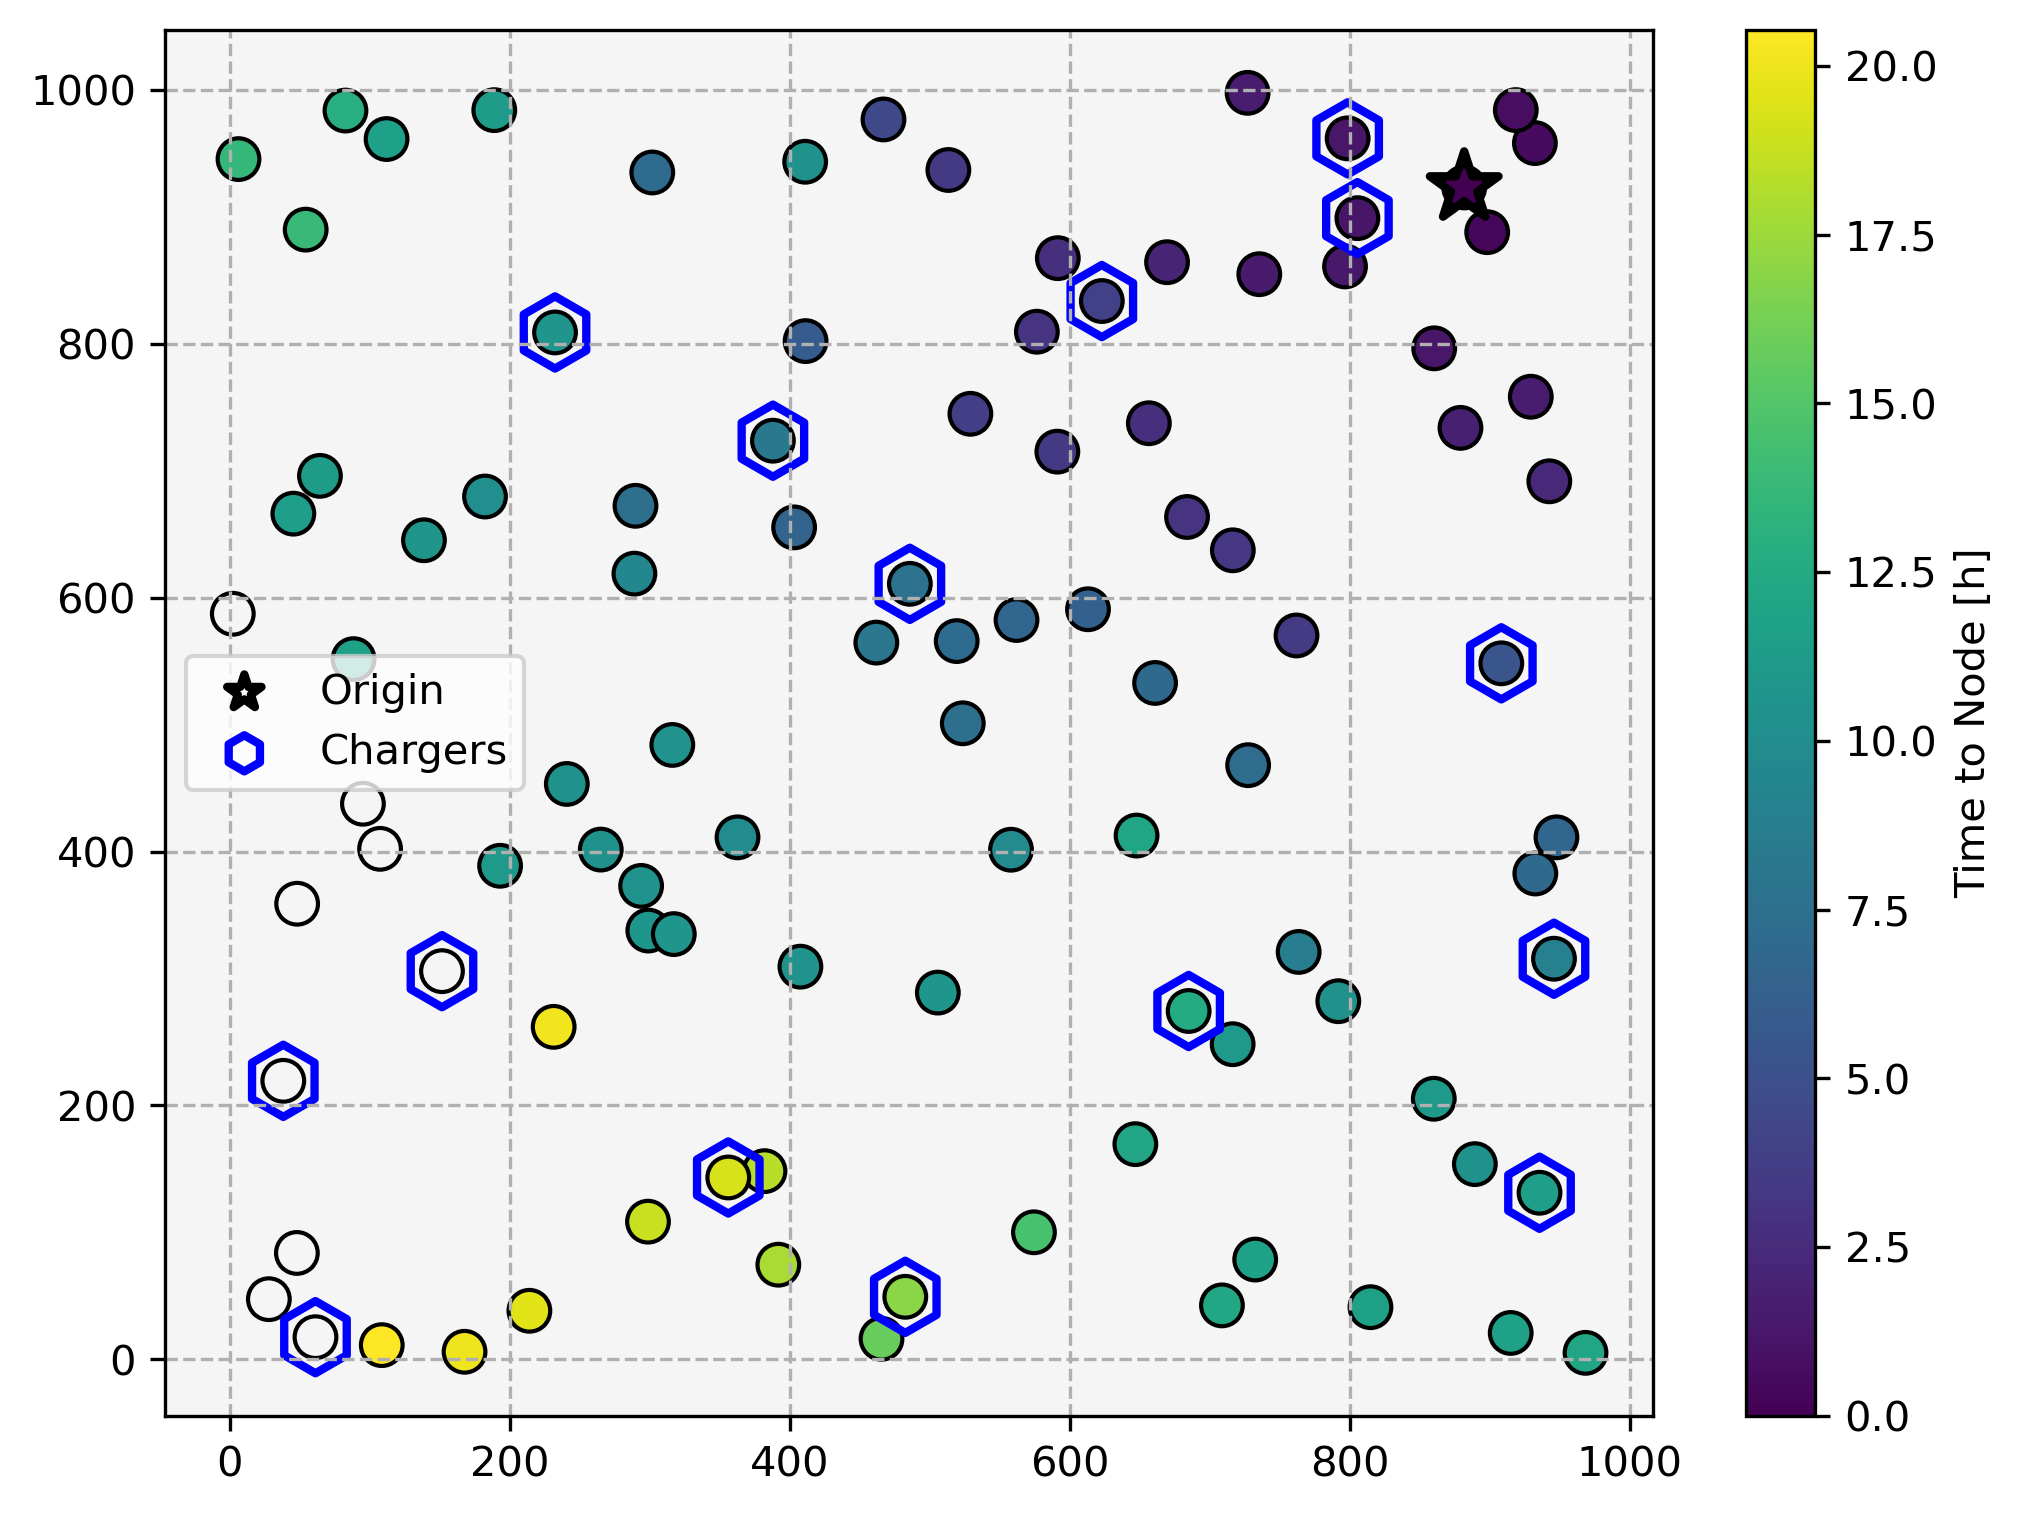
\includegraphics[width = \linewidth]{figs/parameter_factorial_01.png}
		\captionsetup{width=.8\linewidth}
		\caption{High risk tolerance and low charger usability}
	\end{subfigure}
	\begin{subfigure}{.5\linewidth}
		\centering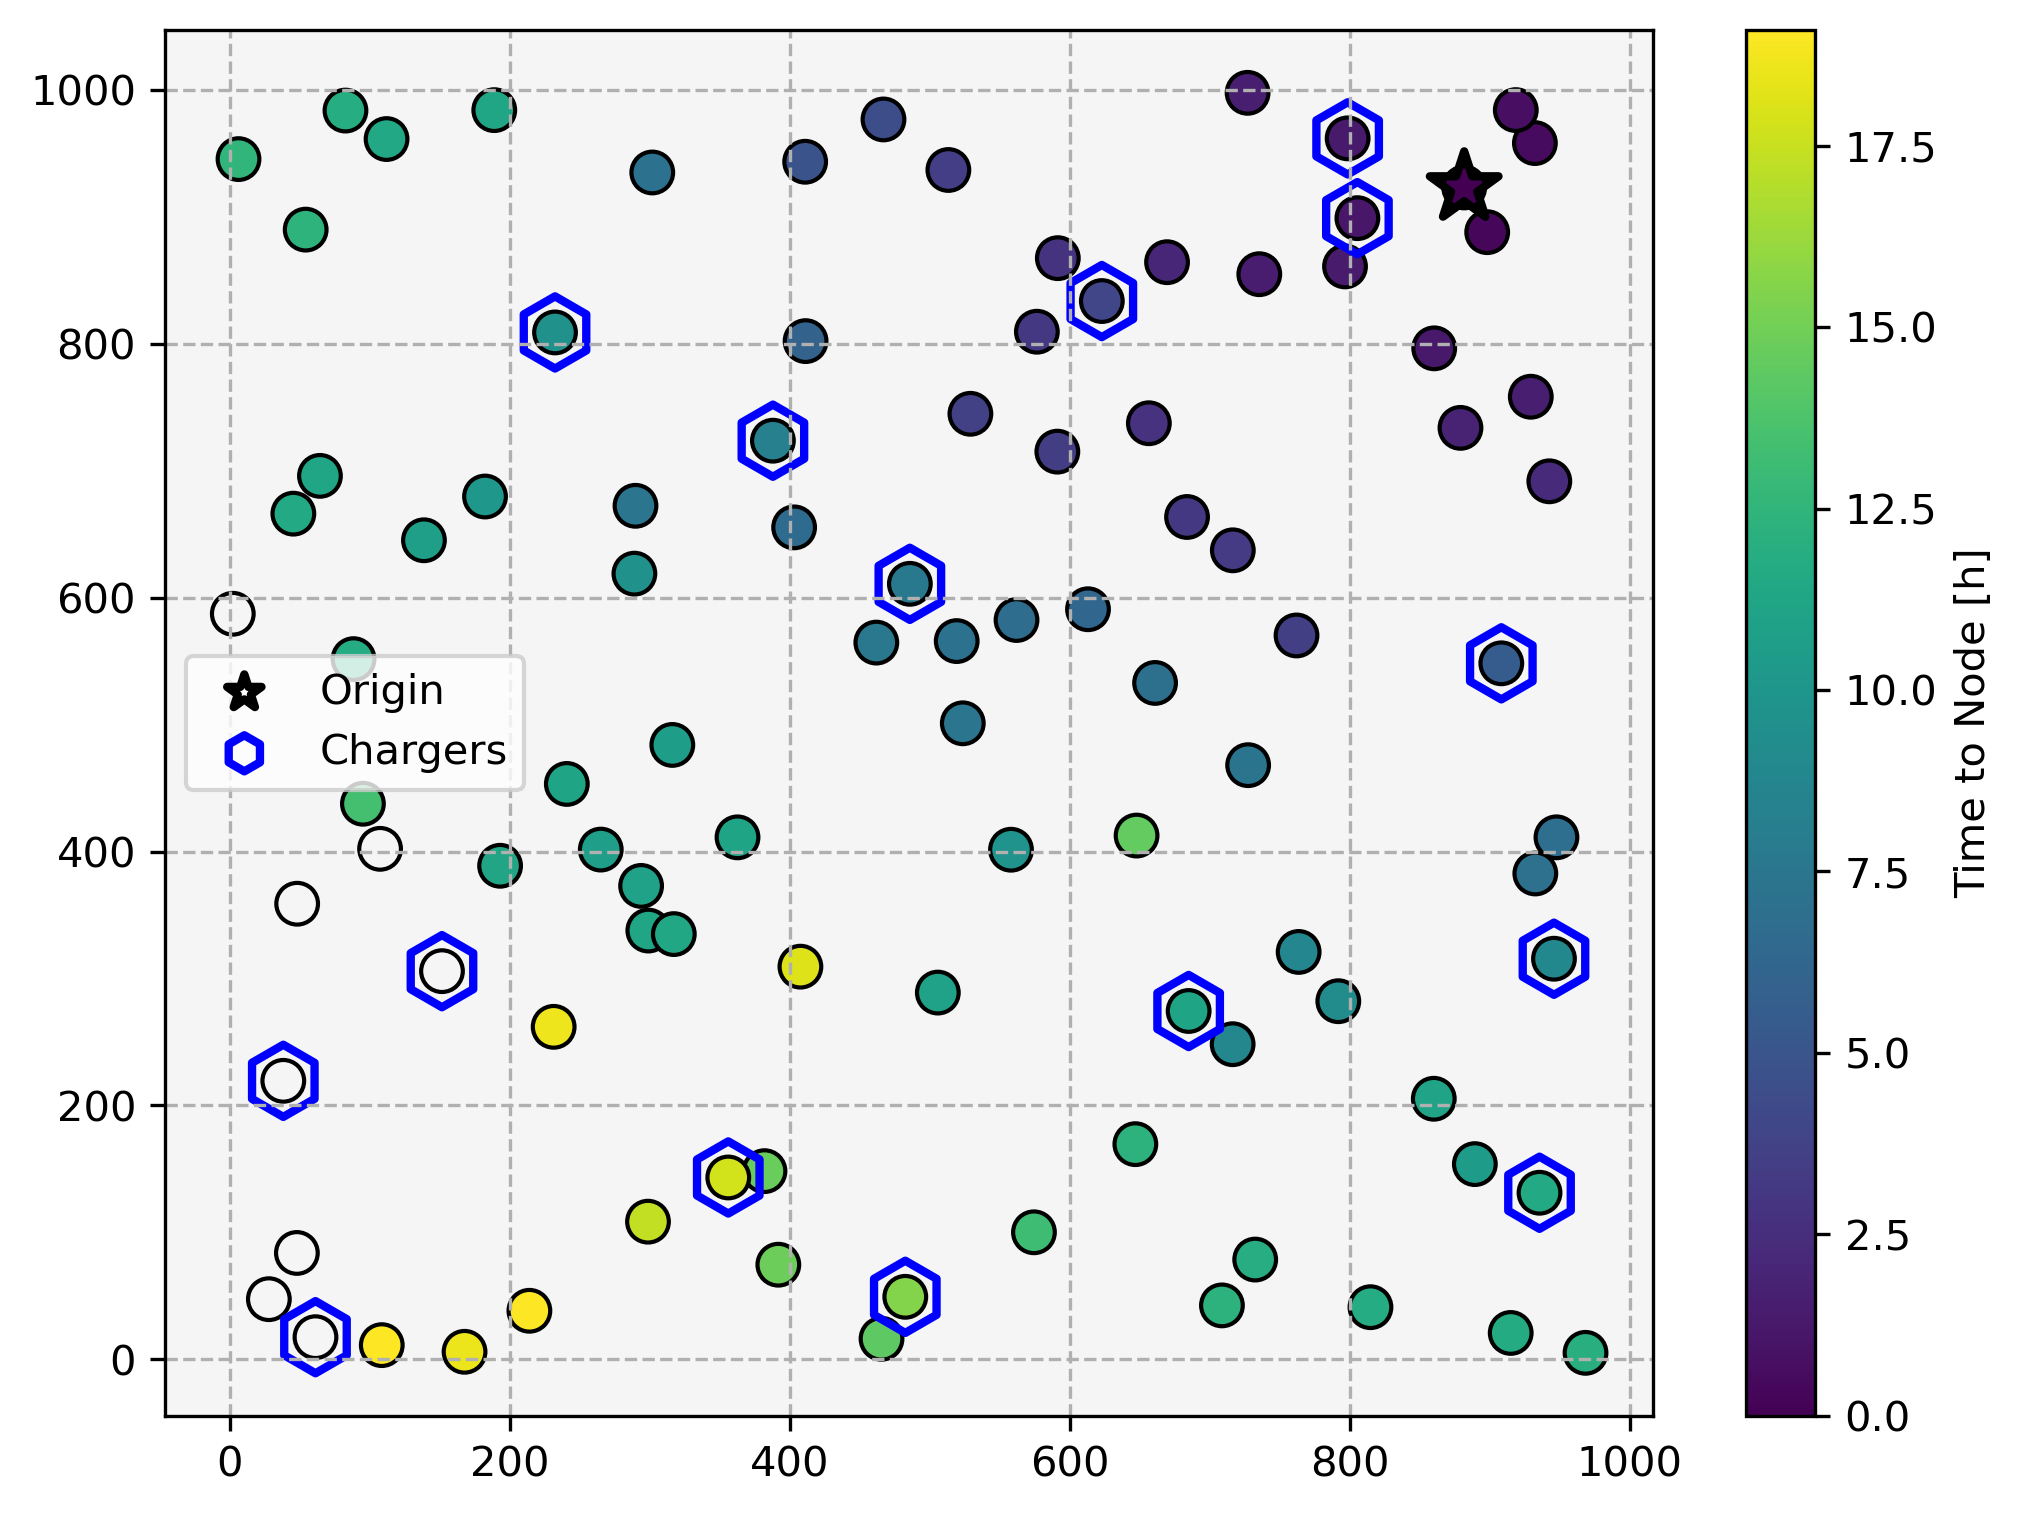
\includegraphics[width = \linewidth]{figs/parameter_factorial_10.png}
		\captionsetup{width=.8\linewidth}
		\caption{Low risk tolerance and high charger usability}
	\end{subfigure}%
	\begin{subfigure}{.5\linewidth}
		\centering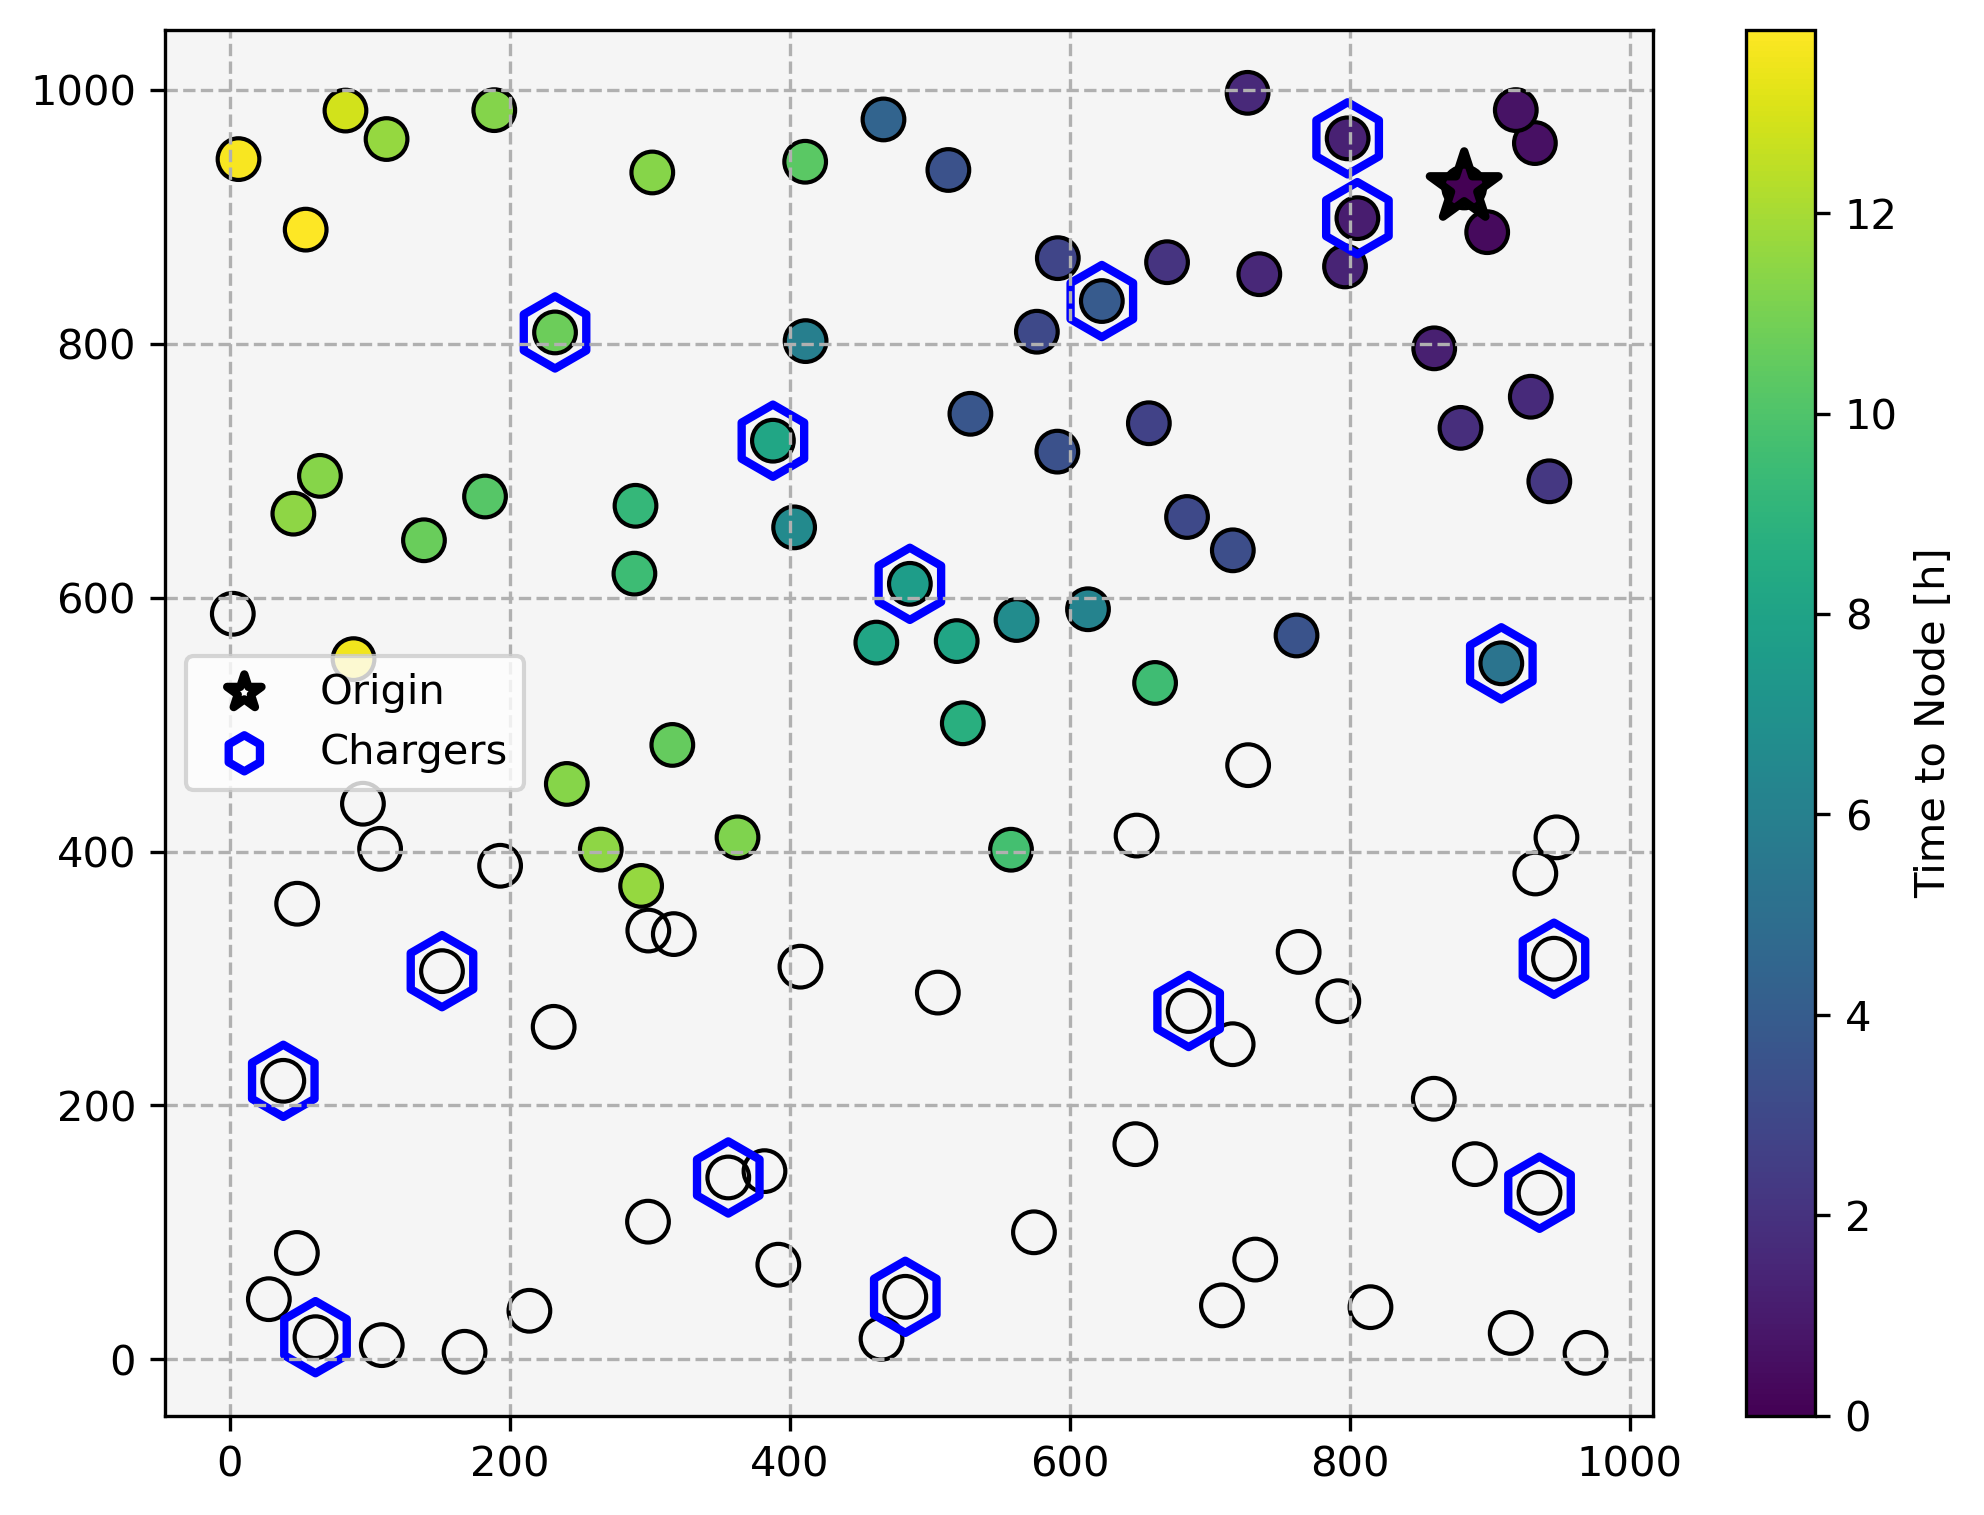
\includegraphics[width = \linewidth]{figs/parameter_factorial_11.png}
		\captionsetup{width=.8\linewidth}
		\caption{Low risk tolerance and low charger usability}
	\end{subfigure}
	\caption{Single-origin expected travel time trees with varying charger reliability and driver risk tolerance}
	\label{fig:routing}
\end{figure}

As seen in Figure \ref{fig:routing}, the effects of poor station reliability and low risk tolerance are additive resulting in worse network utility than either considered individually. Additionally the performance of the network can be computed for \glspl{icev} and \gls{phev} by modeling gasoline as being available at all places for an expected price determined from historical gas prices. By comparing network access for \glspl{bev}, \glspl{phev}, and \glspl{icev} in equivalent situations, the areas where the gap is most and least problematic may be identified.

\subsubsection*{Application}

The framework and tools developed will serve to enable application oriented research to be performed by the team and others. The direct use of the tool will be to evaluate the impacts on network access of station enhancements, additions, and deletions, increased \gls{pev} fleet-share, charger usability rates, and all of the mentioned in combination. The outputs of the project will consist of an open-source software tool and methodological publications followed by application and policy oriented publications and concluded with a comprehensive final report.

\subsection*{Policy and Practice Impact Plan}

\subsubsection*{Relevant Policies and Agency Activity}

Project outputs will be used to inform policies with relation to subsidies and other \gls{evse} installation and operational incentives. The project is, thus, relevant to all agencies involved in such activities including, but not limited to, CalTrans and CEC (and equivalents), US DOE/DOT, and municipal governments. Project outcomes will be most useful to agencies overseeing large areas with substantial transportation corridors. It is highly important that scarce subsidy and incentive funding be spent wisely in order to build out a public \gls{evse} netowrk which can encourage \gls{ev} sales to the point that it is self-sustaining. this goal can be greatly assisted, in the planning stage, using the tools developed herein for alternative comparison and optimization. As such, in addition to publications, open-source tools will be produced.

\subsection*{Engagement Strategy}

Engagement strategy for this project will target public agencies, industry, and academia. The outreach strategy will be three-pronged involving publications and conference presentations, web and social media content, and webinar(s). 

\subsubsection*{Task Descriptions and Deliverables}

The tasks for this project are described in detail below:

\begin{description}
	\item[Task 1:] Literature Review - Compilation of a comprehensive set of related literature concerning driver optimal routing cost hierarchy and risk-attitude and charger usability rates and models.
	\begin{description}
		\item[Deliverable 1A:] Literature review document containing relevant papers, summaries, and overall conclusions.
		\item[Deliverable 1B:] Draft of literature review section of final report.
	\end{description}
	\item[Task 2:] Data Collection - Selection of data sources for required inputs from among those sources mentioned in the data subsection of the methodology section.
	\begin{description}
		\item[Deliverable 2A:] Definition of formatting requirements for input data.
		\item[Deliverable 2B:] Collection and formatting of selected input data.
		\item[Deliverable 2C:] Draft of data review section of final report.
	\end{description}
	\item[Task 3:] Methodology Refinement - The fundamental methodology is, in most aspects, already developed but requires refinement to certain auxiliary elements such as cost models and equivalent-route choice models which will be refined subject to the findings of the literature review.
	\begin{description}
		\item[Deliverable 3A:] Finalize method formulation.
		\item[Deliverable 3B:] Draft of methods section of final report.
	\end{description}
	\item[Task 4:] Tool Development - As with the methodology, the numerical core of the software tool is mostly developed. In order to make the tool broadly usable much front-end and documentation development is necessary.
	\begin{description}
		\item[Deliverable 4A:] Finalize tool numerical method.
		\item[Deliverable 4B:] Develop tool front-end.
		\item[Deliverable 4C:] Develop tool user documentation.
		\item[Deliverable 4D:] Draft of tool development section of final report.
	\end{description}
	\item[Task 5:] Analysis - Following tool development, several proposed policies with relation to \gls{evse} build-out or operational subsidies will be evaluated using the developed framework. General experiments on the roles played by reliability and risk-attitude will also be conducted in furtherance of future policy development. Finally, an equity analysis on the current state of \gls{evse} in California will be conducted.
	\begin{description}
		\item[Deliverable 5A:] Perform proposed analyses using tool.
		\item[Deliverable 5B:] Draft of analysis section of final report.
	\end{description}
	\item[Task 6:] Outreach - Upon completion of tool development at least one methodological publication will be submitted and the tool will be announced via the center website and social media. Publications and announcements will also follow the analysis phase. Team members will engage in Webinars and speak at conferences at various times throughout the project.
	\begin{description}
		\item[Deliverable 6A:] Submit publications based on analyses.
		\item[Deliverable 6B:] Produce website and social media content.
		\item[Deliverable 6C:] Conduct webinar.
	\end{description}
	\item[Task 7:] Final Report - A final report will be composed throughout the duration of the project in stages and will concern motivation, methodology, and analysis. This report will be compiled and edited following the analysis phase and will be the project's final deliverable.
	\begin{description}
		\item[Deliverable 7A:] Compile and edit final report.
	\end{description}
\end{description}

\subsubsection*{Task Schedule with Work Products}

\printbibliography

\end{document}